\documentclass[11pt,a4paper]{article}
\usepackage[UTF8,scheme=plain]{ctex}
\usepackage[margin=2cm]{geometry}
\usepackage{amsmath,booktabs,enumitem,hyperref,graphicx}
\usepackage[labelsep=quad,font=small]{caption}
\usepackage{float}
\usepackage{titlesec}
\usepackage{indentfirst}
\usepackage{placeins}
\titleformat*{\section}{\large\bfseries}
\titleformat*{\subsection}{\normalsize\bfseries}
\titlespacing*{\section}{0pt}{1.4ex plus .3ex}{.7ex}
\titlespacing*{\subsection}{0pt}{1ex plus .2ex}{.5ex}
\setlist{nosep,leftmargin=1.6em}
\linespread{1.16}
\setlength{\parskip}{0.2em}
\setlength{\parindent}{2em}
\setlength{\textfloatsep}{12pt plus 2pt minus 2pt}
\setlength{\intextsep}{10pt plus 2pt minus 2pt}
\hypersetup{colorlinks=true,urlcolor=blue,linkcolor=black}
\AtBeginDocument{\renewcommand{\tablename}{表}\renewcommand{\figurename}{图}}

\title{\bfseries 跨细胞类型的药物响应预测及其误差来源\\[0.3em]
\large 统计学习大作业中期报告}
\author{盛其然 \quad 洪华言 \quad 应硕丞 \quad 樊宇轩}
\date{2026 年 11 月}

\begin{document}
\vspace*{-2.5em}
{\let\newpage\relax\maketitle}
\vspace*{-1.5em}

开题报告提出了四个问题：(一) 如何提高预测精度；(二) 标签是如何生成的；(三) 实验噪声对预测精度构成怎样的上限；(四) 细胞类型特异的响应能否由药物靶点的表达解释。
截至中期，工作主要集中于问题一和问题二：完成了探索性数据分析，建立了统一的验证框架，比较了经典方法与两类神经网络，并阐明了标签的生成机制。
问题三、四目前仅有预实验，其计划在第 6 节说明。

\section{任务与数据}

\subsection{任务定义}
NeurIPS 2023 单细胞扰动竞赛在人外周血单个核细胞中分别加入 144 种小分子药物，24 小时后测定单细胞基因表达，并按细胞类型汇总。
对每个 ``细胞类型 $\times$ 药物'' 组合，主办方通过差异表达分析给出 18{,}211 个基因的标签：
\[
y = \operatorname{sign}(\log\mathrm{FC}) \times \left(-\log_{10} p\right),
\]
其符号表示基因表达变化的方向，绝对值表示变化的统计显著性。因此标签度量的是显著程度，而非变化幅度。

数据包含 6 种细胞类型。NK 细胞和三类 T 细胞（CD4$^+$、CD8$^+$、调节性 T 细胞）几乎覆盖全部药物；
B 细胞和髓系细胞仅公开了 15 种药物和 2 个阳性对照的结果，下文将这 15 种药物称为\textbf{锚点药}。
任务是预测 B 细胞和髓系细胞其余 255 个组合的响应。值得注意的是，这些待预测药物均已在 T/NK 细胞中测定，因此缺失的是\textbf{新细胞类型}上的响应，而非新药物的响应。

评价指标为竞赛采用的 MRRMSE：先对每一行（一个组合）计算跨基因的均方根误差，再对所有行取平均，数值越低越好。
由于各行权重相同，少数响应极强的行可能主导整体误差。

\subsection{探索性分析}
训练集共 614 行，其中包含 12 行阳性对照。

\begin{figure}[!ht]
\centering
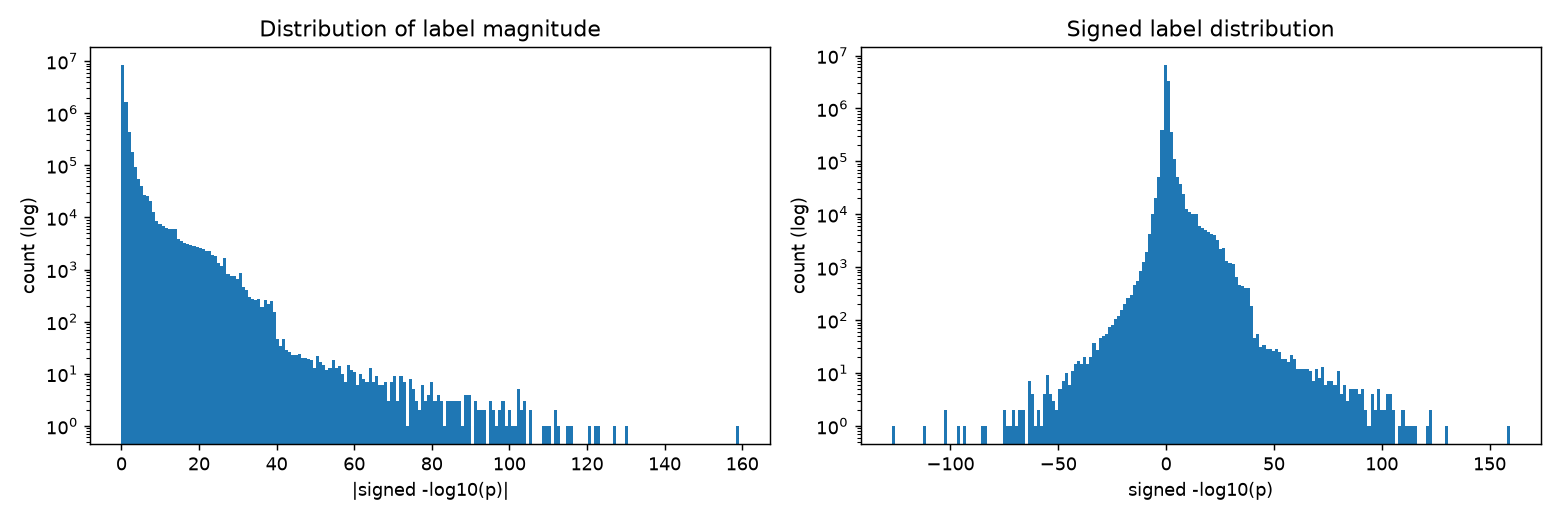
\includegraphics[width=0.75\textwidth]{tm_01_label_distribution.png}
\caption{训练集全部标签值的直方图：602 个药物行（不含阳性对照）$\times$ 18{,}211 个基因，共约 1{,}096 万个值。横轴为标签值，左图取绝对值，右图保留正负号；纵轴为落入每个区间的值的个数，取对数刻度，每高一格表示个数多 10 倍。绝大多数值集中在 0 附近，但仍有少量绝对值超过 100 的极端值。}
\label{fig:labels}
\end{figure}

\begin{figure}[!ht]
\centering
\begin{minipage}[b]{0.5\textwidth}\centering
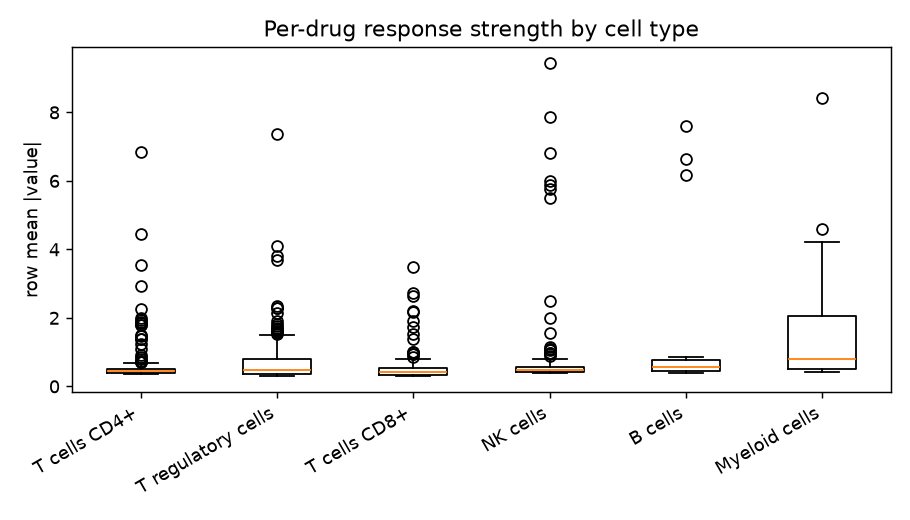
\includegraphics[width=\textwidth]{tm_03_strength.png}\\[-0.3em]
{\small (a)}
\end{minipage}\hfill
\begin{minipage}[b]{0.37\textwidth}\centering
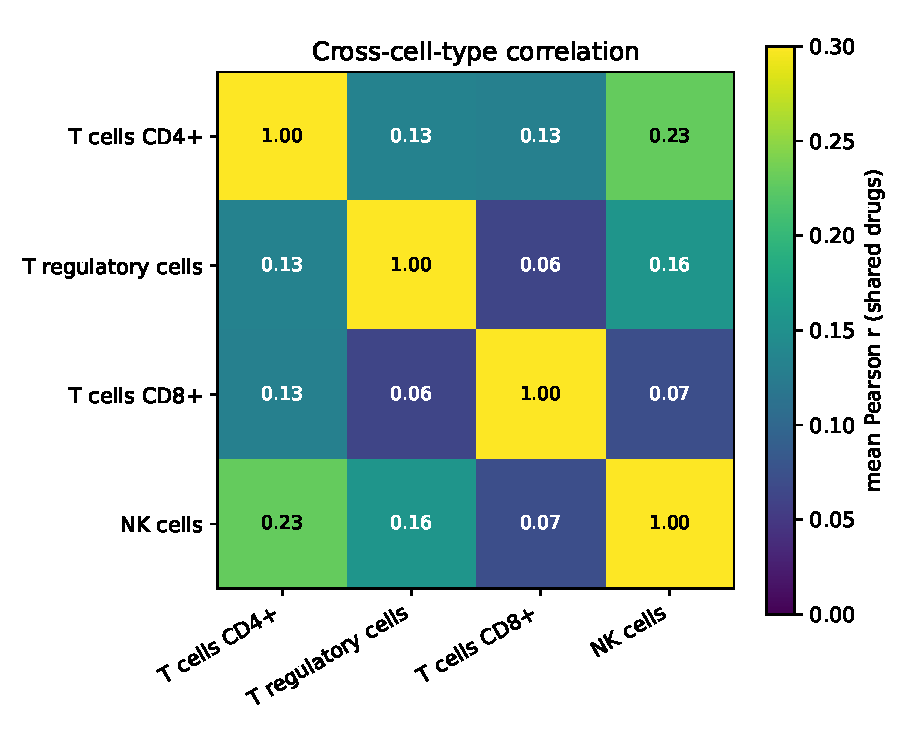
\includegraphics[width=\textwidth]{fig_corr.pdf}\\[-0.3em]
{\small (b)}
\end{minipage}
\caption{(a) 每种药物在各细胞类型中的平均响应强度。(b) 同一种药物在两种 T/NK 细胞类型之间响应的平均 Pearson 相关系数（140 种共有药物，不含阳性对照）。}
\label{fig:strength}
\end{figure}

\textbf{多数标签很弱，少数药物极强。}
图~\ref{fig:labels} 显示，绝大多数标签值接近 0，但存在少量极端值，呈重尾分布。
按行来看（图~\ref{fig:strength}(a)），多数药物的响应很弱，与完全无作用时的噪声水平相当，只有少数具有细胞毒性的药物响应很强。
因此，对大多数行而言，全零预测已接近最优，模型之间的差异主要来自少数强药物。
B 细胞和髓系细胞只有 15 种锚点药，不宜与其他细胞类型直接比较。

\textbf{跨细胞类型的响应呈弱相关。}
图~\ref{fig:strength}(b) 给出同一种药物在两种细胞类型之间响应的平均相关系数。
NK 细胞与 CD4$^+$ T 细胞之间最高（0.23），CD8$^+$ T 细胞与其他细胞之间最低（0.06--0.13）。
相关系数为正，表明可以借助其他细胞类型的响应进行预测；但相关程度较低，表明直接沿用并不可行，模型需要学习如何在细胞类型之间迁移。

\FloatBarrier
\section{标签生成机制}

\subsection{官方流程复现}
每个标签仅对应 3 个孔：实验共有 3 位供体，每种药物在每位供体中各占 1 个孔；溶剂对照（DMSO）和两个阳性对照则各有 48 个孔。
每个样本为一个孔中同一类细胞的计数之和。

我们获取了主办方在竞赛期间使用的脚本，并按其步骤重建了标签：先剔除主办方指定的计数条目，再按 ``孔 $\times$ 细胞类型'' 求和；
随后对每种细胞类型分别用 limma 拟合线性模型，解释变量为药物、供体、板及板上的行，将每种药物与 DMSO 比较，得到 $t$ 值和 $p$ 值。
重建结果与官方训练标签\textbf{逐数值一致}：6 种细胞类型全部吻合，最大绝对差为 $2\times10^{-10}$。

\subsection{训练与测试标签的尺度差异}
主办方说明中指出，训练标签仅用训练样本拟合，测试标签则用全部样本拟合，我们用数据独立验证了这一点。
因此，B 细胞和髓系细胞的锚点标签来自仅含约 185 个样本的拟合（下称小模型），而待预测的测试标签来自样本量大得多的拟合（下称大模型）。
T/NK 细胞没有测试样本，不受此影响。

为量化两者的差异，我们在 T/NK 细胞上进行了模拟：随机抽取 15 种药物，连同对照重新拟合小模型，再与官方标签（即大模型的结果）逐行比较，每种细胞类型重复 31 次。

标签的计算分两步：先求 $t$ 值，即药物效应的估计值除以其标准误，标准误取决于对该基因噪声大小的估计；再按自由度为 $\nu$ 的 $t$ 分布把 $t$ 值换算为 $p$ 值。
大、小模型在这两步中各有一处不同，分别构成差异的两个因素：第二步中的自由度不同（因素一），第一步中的噪声估计不同（因素二）。
两者的作用方式不同：因素一只改变 $t$ 值到标签的换算，主要影响强标签；因素二按比例改变 $t$ 值本身，对强、弱标签都有影响。
因此，按标签强度分档比较（图~\ref{fig:ratio}），可以将两者区分开来。

\begin{figure}[!ht]
\centering
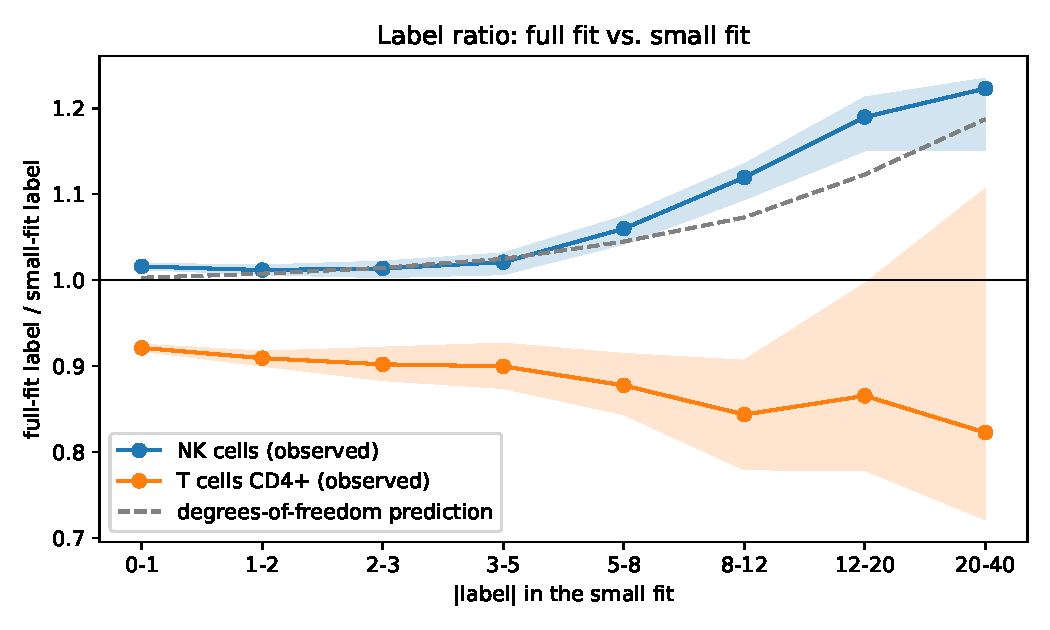
\includegraphics[width=0.48\textwidth]{fig_ratio.pdf}
\caption{同一批孔的标签在 ``只用 15 种药拟合''（小模型）与 ``用全部药拟合''（大模型）之间的比值，按小模型标签的绝对值分档。阴影为按药物重抽样的 95\% 区间，虚线为只考虑自由度时的理论预测。}
\label{fig:ratio}
\end{figure}

\textbf{因素一：自由度。} $p$ 值由 $p = 2P(T_\nu > |t|)$ 得到，其中 $\nu$ 为 limma 经验贝叶斯调整后的总自由度（残差自由度与先验自由度之和）。
小模型的 $\nu$ 约为 168，大模型约为 424。自由度越小，$t$ 分布的尾部越厚，相同 $t$ 值对应的 $-\log_{10}p$ 越小。
为单独考察这一因素，我们作如下假设：(1) 两次拟合得到的 $t$ 值相同，即暂不考虑因素二；(2) $\nu$ 对所有基因取同一值；
(3) $|t|$ 较大而 $t^2/\nu$ 较小，可对 $t$ 分布的尾部展开并只保留 $1/\nu$ 的一阶项。记小模型的标签为 $y$，则
\[
\frac{y_{\text{大}}}{y_{\text{小}}} \approx 1 + \ln 10 \cdot y \left(\frac{1}{\nu_{\text{小}}} - \frac{1}{\nu_{\text{大}}}\right) \approx 1 + 0.008\,y .
\]
在假设 (1)(2) 下精确计算（不作展开），$y=10$ 时两者相差约 7\%，$y=40$ 时约 32\%，与上式接近；对 $|y|<2$ 的绝大多数基因，差异不足 2\%。

图~\ref{fig:ratio} 中的虚线即为假设 (1)(2) 下的精确计算结果。
NK 细胞的实测曲线在弱标签处接近 1，在强标签处随虚线上升，说明其差异主要来自因素一。
CD4$^+$ T 细胞的曲线则在所有分档上都低于 1：在弱标签处因素一可以忽略，偏离只能来自 $t$ 值本身的变化，即假设 (1) 不成立，这就是因素二。

\textbf{因素二：噪声估计的样本构成。}
每种药物在每种细胞中仅有 3 个孔，不足以可靠地估计噪声。因此 limma 先用线性模型（药物、供体、板、行）拟合同一细胞类型的全部样本，
将各样本中模型无法解释的部分（残差）汇总，估计每个基因的噪声方差，并由所有药物共用这一估计。
由此，噪声估计反映的是\textbf{参与拟合的全部样本}的平均噪声水平。

两次拟合的样本构成差别很大。对照孔（溶剂对照和两个阳性对照）各有 48 个，而每种普通药物仅有 3 个。
小模型只包含 15 种药物，对照孔约占样本的 78\%；大模型包含全部药物，对照孔仅占约 25\%。
若对照孔与普通药物孔的噪声相同，样本构成不会影响结果，但实际情况并非如此。
我们按样本分组，比较各组残差的实际方差与模型预期的方差（图~\ref{fig:noise}(a)）：
在 CD4$^+$ T 细胞中，对照孔的噪声方差比普通药物孔低约 15\%，因此小模型低估了噪声，$t$ 值偏大，大、小模型的标签之比低于 1，这正是图~\ref{fig:ratio} 中 CD4$^+$ 曲线整体低于 1 的原因；
在 CD8$^+$ T 细胞和调节性 T 细胞中情况相反，阳性对照孔的噪声方差比普通药物孔高约 40\%（主要来自阳性对照之一 Belinostat），比值高于 1；NK 细胞中各组噪声接近，比值接近 1。
据此可以推算标签之比。这一推算只计入了分组噪声差异，没有计入自由度；为使比较成立，我们只在弱药物行上进行比较，其标签绝对值大多小于 2，因素一的影响在 1\% 左右，可以忽略。
推算值与模拟实测值基本吻合（图~\ref{fig:noise}(b)），说明弱标签上的差异确实来自因素二。

综合两个因素：在弱标签上，差异主要来自因素二，其方向和大小随细胞类型而异；在强标签上，因素一叠加于其上，且总是使大模型的标签更大。

\begin{figure}[!ht]
\centering
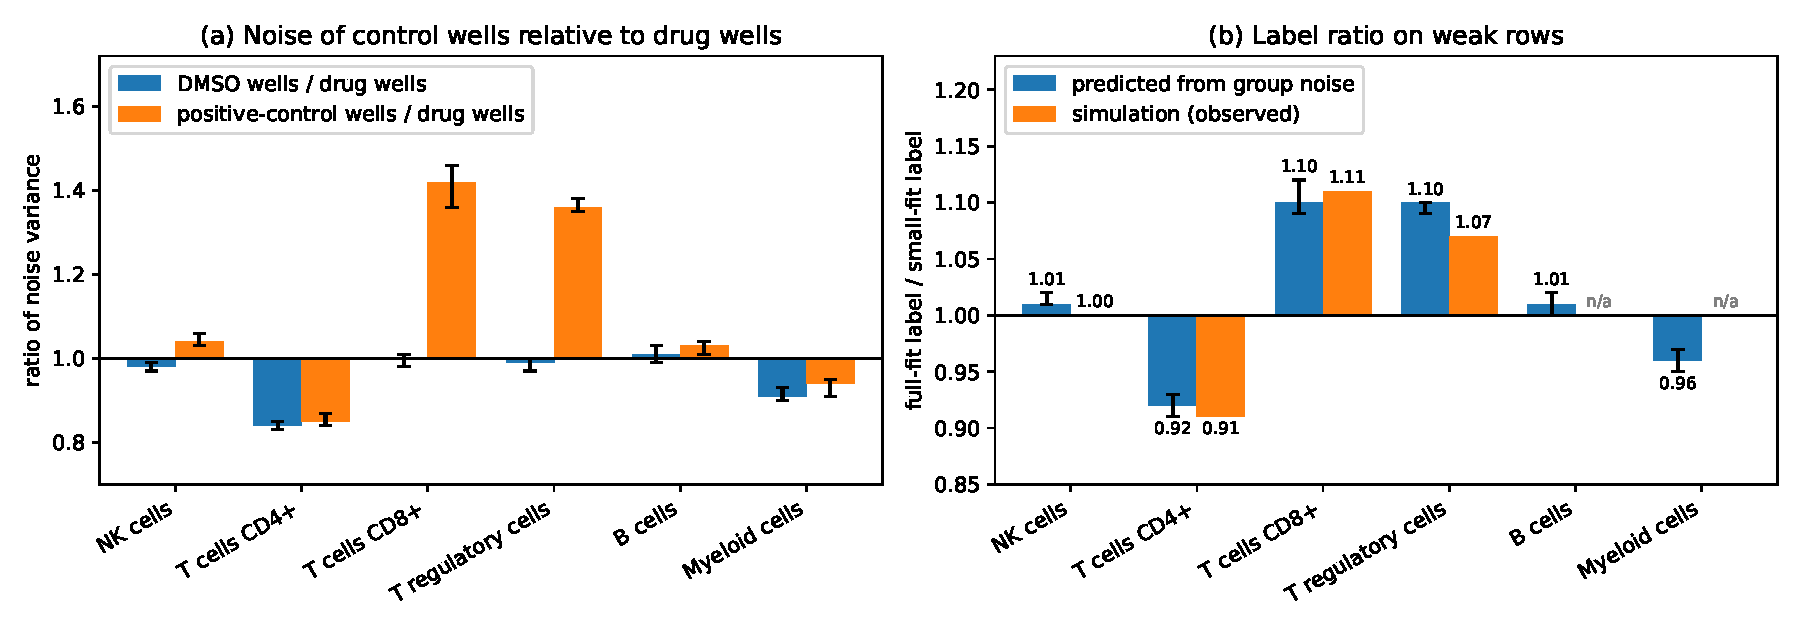
\includegraphics[width=0.76\textwidth]{fig_noise.pdf}
\caption{(a) 对照孔与普通药物孔的噪声方差之比（残差方差相对模型预期方差，取 3000 个基因的中位数；误差线为对基因重抽样的 95\% 区间）。
(b) 由 (a) 中的分组噪声差异推算的标签之比（蓝）与模拟实测值（橙），只统计弱药物行。B 细胞和髓系细胞没有测试样本，无法进行模拟。}
\label{fig:noise}
\end{figure}

噪声偏高的样本为何在不同细胞类型中落在不同的组？limma 在估计噪声前，会依据每个样本中每个基因的表达量赋予权重，其前提是表达量越高、噪声越小。
我们发现这一前提在两类样本上不成立：仅含 1--5 个细胞的样本，以及强毒性药物处理的孔。
Belinostat 使调节性 T 细胞几乎全部消失，并使 CD8$^+$ T 细胞的数量在不同供体之间差异悬殊，因此这两类细胞的异常样本集中于阳性对照组；
CD4$^+$ T 细胞数量充足、受影响较小，其异常样本则分散在普通药物组中。这解释了 CD4$^+$ 与 CD8$^+$ T 细胞偏移方向相反的现象。

\subsection{对预测的影响}
因素二的推算只需训练样本，因此可直接用于 B 细胞和髓系细胞（图~\ref{fig:noise}(b)）：B 细胞的标签之比约为 1.01，可以忽略；髓系细胞约为 0.96，即弱标签上锚点反而略偏大。
由此推断，两者的锚点标签与测试标签之间的差异主要来自因素一，集中在强药物的极显著基因上。

为检验这一差异是否影响预测，我们在协议 A 中将目标细胞的锚点标签替换为小模型标签，使验证中锚点与待预测行的尺度关系与真实任务一致。
模型选用局部核岭回归（见第 4.2 节），它只以锚点为标签，对锚点尺度最为敏感。锚点标签分三种：小模型标签，不作校正；按因素一的公式换算到大模型尺度；直接使用大模型标签，作为标签尺度完全对齐的参照。

在整体指标上，三者没有可检测的差别：即使使用大模型标签参照，各细胞类型的 MRRMSE 也未改善（变化在 $0.000$ 到 $+0.012$ 之间，按行配对自助法的 95\% 置信区间均包含 0）。
但整体指标主要由弱元素决定，而因素一只作用于强元素。因此我们单独考察待预测行中真值绝对值大于 10 的元素，以沿真值方向的平均误差衡量预测幅度的偏差（表~\ref{tab:strong}）。

\begin{table}[!ht]
\centering\small
\caption{局部核岭回归在强元素（真值 $|y|>10$）上沿真值方向的平均误差。负值表示预测幅度偏小；校正一列为相对不校正的变化，正值表示低估减轻，括号内为按行重抽样的 95\% 区间。}\label{tab:strong}
\begin{tabular}{@{}lccc@{}}
\toprule
细胞类型 & 不校正 & 按自由度换算 & 大模型标签参照 \\
\midrule
NK & $-10.5$ & $+0.96$ $[+0.15, +1.59]$ & $+1.24$ $[+0.16, +2.10]$ \\
CD4$^+$ T & $-11.5$ & $+0.72$ $[+0.07, +1.05]$ & $+0.13$ $[-0.21, +0.80]$ \\
CD8$^+$ T & $-15.9$ & $+0.43$ $[+0.01, +0.89]$ & $+2.25$ $[+0.01, +4.74]$ \\
调节性 T & $-11.2$ & $+0.02$ $[+0.01, +0.12]$ & $+0.56$ $[+0.11, +0.58]$ \\
\bottomrule
\end{tabular}
\end{table}

在这些位置上，模型的预测幅度普遍严重偏小；按自由度换算后，四种细胞的低估均显著减轻，与理论一致。
在与 B 细胞情形最接近的 NK 细胞上，换算获得了大模型标签参照约八成的改善。CD4$^+$ T 细胞上换算优于大模型标签参照，因为大模型标签还包含方向相反的因素二；CD8$^+$ 和调节性 T 细胞的锚点中强元素很少，换算几乎不改动标签。

由此得到的结论是：标签尺度差异确实存在，并在强元素上造成可测量的低估，按自由度换算可以部分纠正。
但它只占强元素低估量的十分之一左右，主要部分来自模型对强响应的整体收缩；加之强元素只占待预测元素的约 1.5\%，在当前局部核岭回归和四个模拟任务中，校正未显示整体指标的稳定改善，尚不能据此外推真实测试集上的改善幅度。

\section{验证设计}

课程要求不得使用测试标签，因此需要自行构造验证集。验证应尽量模拟真实任务：目标细胞只提供 15 个锚点，需预测其余药物的响应。

我们采用两种协议，共 34 个验证折（表~\ref{tab:protocols}），本文所有内部分数均在这组折上计算。

\begin{table}[H]
\centering\small
\caption{验证协议（共 34 折）}\label{tab:protocols}
\begin{tabular}{@{}lp{0.62\textwidth}l@{}}
\toprule
协议 & 做法 & 折数 \\
\midrule
A & 依次将一种 T/NK 细胞视为新细胞，仅保留其 15 个锚点和 2 个阳性对照（真实任务中同样可见），预测其官方测试药物 & 4 \\
V & 在 B 细胞和髓系细胞上，每次留出一个锚点进行预测 & 30 \\
\bottomrule
\end{tabular}
\end{table}

两种协议各有所长：协议 A 的任务结构与真实任务一致，但细胞类型不同；协议 V 的细胞类型一致，但预测对象是锚点，其中少数强毒性药物的误差很大，容易主导结果。
因此我们在协议 V 中另行统计\textbf{弱锚点}，即在其他细胞中响应较弱的锚点，它们与大多数测试药物更为接近。

\textbf{综合指标}取协议 A 和协议 V 弱锚点各自相对第一版核岭回归的误差比的平均值（第一版核岭回归记为 1，越低越好）。

\section{模型与结果}

\subsection{经典方法}
我们系统比较了 20 余种经典方法。输入特征约 260 维，由三部分组成：药物 SMILES 字符串的 $n$-gram 指纹（经降维）、
药物签名，以及细胞签名（目标细胞锚点药的平均响应）。所有签名均只用训练折中可见的行计算。
方法包括线性回归、岭回归、偏最小二乘、近邻回归、核岭回归、降秩回归、随机森林等树模型、sklearn 神经网络，以及先对输出做主成分分析再回归的各种组合，并对其中若干方法进行了等权集成。

结论高度一致：\textbf{这些方法均接近或不如全零预测}。接入统一框架的几种经典方法在协议 A 上的 MRRMSE 介于 1.01 与 1.13 之间，而全零为 1.006。
仅将输出约束为低秩的方法（降秩回归、主成分回归）略有改善。

此外还有以下几项负面结果：
\begin{itemize}
\item \textbf{目标自编码器}：先用自编码器将响应压缩到低维，再预测该低维表示。其效果不如线性的截断奇异值分解。训练数据仅约 440 行，非线性压缩的参数过多，将噪声也一并拟合。
\item \textbf{CP 张量分解}：将数据视为 ``细胞 $\times$ 药物 $\times$ 基因'' 的三维张量进行分解。其效果甚至不如仅使用药物签名。原因在于新细胞的因子只能由 15 个锚点估计，其中少数强毒性药物主导了估计，得到的尺度存在系统偏差。
\item \textbf{随机 K 折 bagging}：每次仅用 2/3 的数据训练，再对多次结果取平均。各折结果均变差，因为数据量过小，舍弃数据造成的信息损失超过了方差降低带来的收益。
\end{itemize}

\subsection{锚点迁移模型}
经典方法未能专门利用目标细胞自身的锚点，锚点迁移模型即从这一点出发。

\textbf{局部核岭回归。} 对每个目标细胞单独拟合，仅以其 15 个锚点为标签。预测值由三部分相加：
目标细胞锚点的逐基因中位数（作为参照）；药物在 T/NK 细胞中的平均偏移，经降维去噪并乘以收缩系数；
以及依据查询药物与各锚点在 T/NK 细胞中的相似度，借用锚点的残差。
这是\textbf{第一个稳定优于全零}的方法，并且在强药物上表现最好。因此我们以它的第一版作为内部评估的基准，综合指标即以第一版核岭回归的分数为 1。

\textbf{神经网络。} 将标签降至 64 维（截断奇异值分解），以细胞类型和药物的留一平均编码作为输入，由多层感知机输出低维坐标，损失函数采用原 18{,}211 维空间的 MRRMSE（包含降维时被截断部分的残差）。
在此基础上，我们提出了两项改进：
\begin{itemize}
\item \textbf{I1 类比编码}：利用在其他细胞中与该药物相似的锚点在目标细胞中的表现，构造一个额外输入，相当于将核岭回归的思想引入网络输入。
\item \textbf{I2 幅度输出头}：将输出分解为方向和幅度两部分，幅度随药物在其他细胞中的强度增大，并按细胞类型缩放。原网络的预测幅度明显不足（在强锚点上仅为真值的约四成），I2 弥补了这一不足。
\end{itemize}
\textbf{融合模型。} 网络在弱药物上更准，局部核岭回归在强药物上更好，两者互补。
我们将两个网络（带幅度输出头的网络，以及同时含 I1 和 I2 的网络）与局部核岭回归按固定权重 0.4、0.4、0.2 加权平均，得到\textbf{融合模型}，它是目前的最终模型。

\subsection{嵌入表示网络}
另一条思路不使用人工构造的特征，而是为每种细胞类型和每种药物各学习一个 128 维的向量（embedding），经全连接网络输出 25 维低秩表示，再还原到全部基因。
训练目标是低维坐标上的逐行 RMSE（不含被截断部分的残差），最终按原空间的 MRRMSE 评估。
变体包括加入药物签名的混合模型，以及以 SMILES 字符串为输入的一维卷积网络 \textbf{SMILES-CNN}（本节唯一使用化学结构的模型）。

调参中，学习率与 embedding 维度影响最大，逐行 RMSE 明显优于普通均方误差；SMILES-CNN 与纯 embedding 网络效果相当，即在当前已见药物的迁移任务中，SMILES 编码未显示稳定的额外收益。
这一方向的早期提交中，官方私有榜分数从经典方法的 0.885 降到调参后 embedding 网络的 0.762。

\subsection{统一框架下的比较}
所有模型均在同一验证框架下评估，表~\ref{tab:main} 列出各类方法中有代表性的模型；其官方分数均来自同一框架下生成的提交，以保证与内部分数对应同一个模型。

\begin{table}[!ht]
\centering\small
\caption{统一框架下代表性模型的结果（均为越低越好）。全部模型的结果见代码仓库。}\label{tab:main}
\setlength{\tabcolsep}{4pt}
\begin{tabular}{@{}llccccc@{}}
\toprule
模型 & 类别 & 协议 A & 协议 V（弱锚点） & 协议 V（全部） & 综合指标 & 私有榜 / 公开榜 \\
\midrule
全零 & 基线 & 1.006 & 1.202 & 2.853 & 1.052 & 0.902 / 0.666 \\
经典集成 & 经典方法 & 1.012 & 1.244 & 2.164 & 1.073 & 0.878 / 0.637 \\
\midrule
局部核岭回归 & 锚点迁移 & 0.946 & 1.133 & 1.731 & 0.990 & 0.799 / 0.594 \\
神经网络 + I2 & 锚点迁移 & 0.923 & 1.018 & \textbf{1.540} & 0.929 & 0.735 / 0.577 \\
\textbf{融合模型} & 锚点迁移 & 0.919 & \textbf{1.015} & 1.551 & \textbf{0.925} & \textbf{0.734} / 0.573 \\
\midrule
embedding 网络 & 嵌入表示 & 0.912 & 1.073 & 1.643 & 0.946 & 0.772 / 0.573 \\
SMILES-CNN & 嵌入表示 & \textbf{0.899} & 1.052 & 1.666 & 0.931 & 0.762 / \textbf{0.572} \\
\bottomrule
\end{tabular}
\end{table}

由表~\ref{tab:main} 可得以下结论：
\begin{itemize}
\item \textbf{经典方法在内部验证上同样不如全零}，与早期实验的结论一致；在官方私有榜上，经典集成仅略优于全零（0.878 对 0.902）。
\item \textbf{能够利用锚点或低秩结构的模型均明显优于全零}。两类网络中最好的模型在综合指标上接近：融合模型为 0.925，SMILES-CNN 为 0.931。
\item \textbf{两类网络各有所长}：embedding 网络和 SMILES-CNN 在协议 A 上最好，锚点迁移网络在协议 V 的弱锚点和强锚点上更好。逐行配对比较的置信区间均包含 0，目前的差异在统计上尚不显著。
\item 官方私有榜上表现最好的是融合模型（0.734），其次为带幅度输出头的网络（0.735）；嵌入表示网络中，SMILES-CNN（0.762）好于 embedding 网络（0.772），并在公开榜上最好（0.572）。作为参照，竞赛私有榜第一名为 0.729，中位数为 0.793。
\end{itemize}

\section{内部验证与官方评分的一致性}

获得官方分数后，可以检验内部验证的可靠性。我们选取全部 21 个有官方分数的学习型模型（不含朴素基线，包括未列入表~\ref{tab:main} 的模型），计算各项内部指标与官方分数的 Spearman 秩相关（表~\ref{tab:corr}）。

\begin{table}[!ht]
\centering\small
\caption{内部指标与官方分数的秩相关（21 个模型）}\label{tab:corr}
\begin{tabular}{@{}lccc@{}}
\toprule
内部指标 & 与私有榜 & 与公开榜 & 两两排序与私有榜一致的比例 \\
\midrule
协议 A & 0.72 & 0.87 & 77\% \\
协议 V（弱锚点） & \textbf{0.95} & 0.73 & \textbf{92\%} \\
协议 V（全部锚点） & 0.84 & 0.86 & 83\% \\
综合指标 & 0.93 & 0.86 & 90\% \\
\bottomrule
\end{tabular}
\end{table}

\textbf{协议 V 的弱锚点项与私有榜最为一致}，这与预期相符：私有榜的 79 种药物大多为弱药物，而该项衡量的正是在 B 细胞和髓系细胞上预测弱药物的能力。
协议 A 与私有榜的相关最弱。例如 embedding 网络在协议 A 上略优于融合模型，但在弱锚点上明显较差，官方私有榜与弱锚点一致（0.772 对 0.734）。
可见以 T/NK 细胞模拟新细胞所得的结论，迁移到 B 细胞和髓系细胞时并不总是成立。

需要说明两点。第一，几个明显较差的经典方法扩大了分数范围，使相关系数偏高；只考察较强的 15 个模型时，弱锚点项与私有榜的秩相关为 0.88，协议 A 仅为 0.29。
第二，官方分数仅用于事后检验已经固定的模型，我们没有据此修改综合指标，否则相当于间接利用测试标签选择模型。

\section{后续工作}

\begin{itemize}
\item \textbf{融合两类模型。} 锚点迁移模型与嵌入表示网络在不同协议上各有优势，且各验证折上的预测均已保存，可直接检验两类模型的融合是否有效。
\item \textbf{提高稳定性。} 仅用单个随机种子的全连接网络，在改变训练数据的构造方式后，私有榜分数变化可超过 0.2。后续所有网络均应采用多个随机种子，并报告种子之间的波动。
\item \textbf{问题三（噪声上限）。} 由于已能精确复现标签流程，可将 DMSO 孔随机分组作为 ``假药物''，得到与真实标签同尺度的纯噪声标签，据此估计弱药物行的误差下限，并将各模型的误差分解为方向、幅度和噪声三部分。
\item \textbf{问题四（靶点表达）。} 预实验发现，髓系细胞特异性最强的两种锚点药均为 AXL 抑制剂，而 AXL 仅在髓系细胞中表达。下一步将整理靶点注释，用置换检验考察靶点表达与响应特异性的关系。
\end{itemize}

\end{document}
